\section{PROBLEMS DETECTED AND SOLUTIONS IMPLEMENTED}
This chapter describes problems that appeared during the development of the project as well as solutions implemented.
\subsection{Debug mode}
When trying to work with the debug mode of Mbed Studio, and in an early version of the project, the debugger wasn't launching. The error can be seen in the next figure.
\begin{figure}[H]
    \centering
    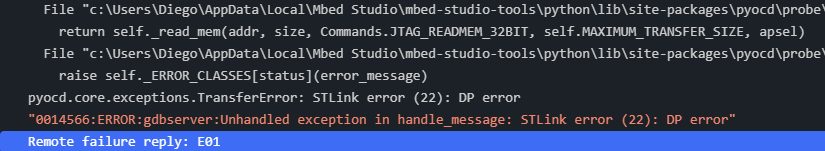
\includegraphics[width=0.8\textwidth]{images/6/Debug Problem.png}
    \caption{Debug error}
    \label{fig:debugProblem}
\end{figure}
As the project involved multiple modules, communication interfaces and threads. Some time was spent understanding the error and getting the debugger to work.

After research and trial and error. The solution was found. The L072CZ connects the \texttt{PA\_13} and \texttt{PA\_14} pins directly to the SW debugger of the ST Link as presented in the \autoref{fig:debugPins}. 
\begin{figure}[H]
    \centering
    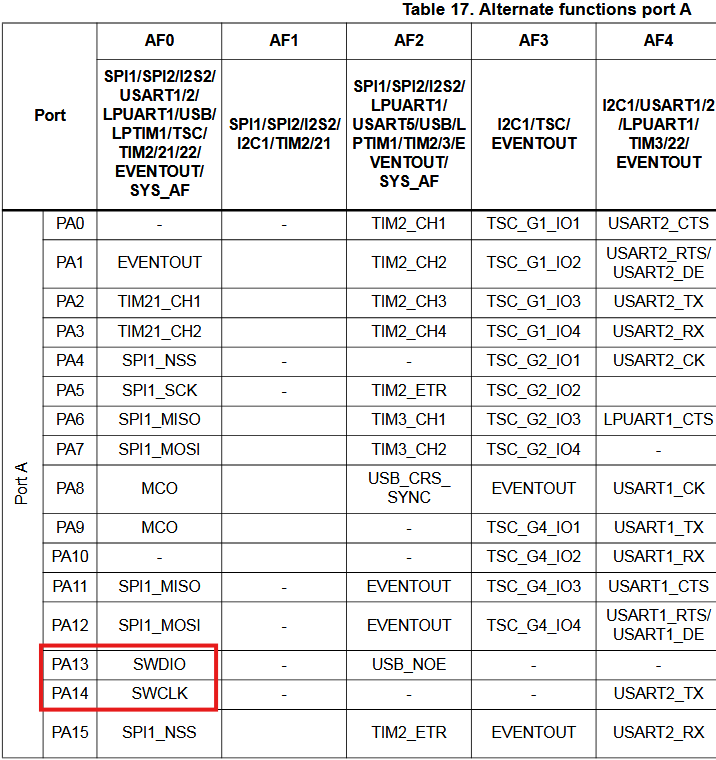
\includegraphics[width=0.6\textwidth]{images/6/DebugPins.png}
    \caption{Pins used by the SW debugger}
    \label{fig:debugPins}
\end{figure}
When the RGB Led was started, the alternate function of the pin is overwritten, and the connection to the debugger is lost. To solve this, a macro was defined in the system, that can be commented and allow the RGB led module to work with all the colors.

\subsection{Problems with the color sensor}
The color sensor was configured to implement the requirements of the advanced mode in regards to the interruptions generation. The configuration was properly validated with a logical analyzer.

When everything was configured, no observable change in the logical level of the interrupt pin was seen.

To see the problem in a modular way, an external implementation\cite{TCS3472_I2CClasswhich} of an interface to the sensor was used. When trying to enable the interruptions, the code returned a 0, indicating that 
a problem had occurred.
\subsection{Problems with the accelerometer}
When working with the accelerometer, the data obtained wasn't being read properly. When inspected with the logical analyzer, the data that was being sent back to the \acrshort{mcu} was fixed. This can be seen in the next figure.
\begin{figure}[H]
    \centering
    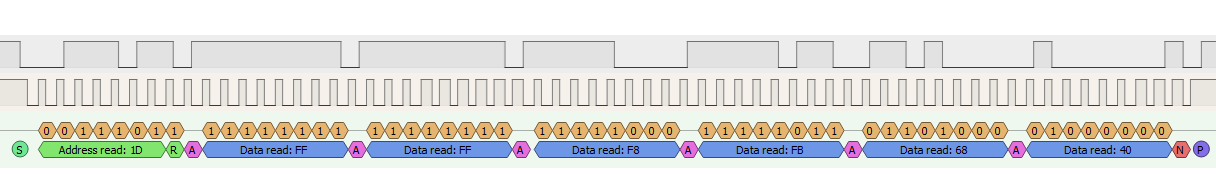
\includegraphics[width=0.9\textwidth]{images/6/accProblem.png}
    \caption{Accelerometer fixed data without repeated start}
    \label{fig:accProblems}
\end{figure}
After some research and, as vaguely indicated by the dataset\cite{MMA8451Q1a}, the sensor expects repeated start between write and read operations.
\subsection{Fault problem}
When implementing and testing the GPS, and in the final week, some HardFaults were seen in the project. After talking with the teachers of the subject, the main suspect of this problem were 
the change done in the default stack size of the Mbed-OS threads. In this case, one of the main possible conflict point is the GPS thread.

As the GPS thread performs parsing on strings, the amount of memory needed by the thread is more than expected, to solve this, more stack size was assign to the GPS thread.